%Styles
\tikzstyle{ground}=[color=gray,postaction={draw,decorate,decoration={border,angle=-45,amplitude=0.2cm,segment length=2mm}}]
\tikzstyle{actuator} = [draw=blue!50!black ,fill=blue!50!black!50!white, thick, rectangle, inner sep=0,minimum height=0.6cm, minimum width=0.2cm, node distance=1.8cm]
\tikzstyle{spring} = [thick,green!50!black,decorate,decoration={snake,amplitude=3,segment length=10}]
\tikzstyle{wheel} = [thick,orange,decorate,decoration={coil,aspect=0.7,amplitude=5}]
\tikzstyle{cart} = [rectangle, inner sep=0,minimum height=0.8cm, minimum width=1.5cm, node distance=1.8cm, path picture={ 
      \draw[thick] ([yshift=0.12cm, xshift=0.3pt] path picture bounding box.south west) rectangle ([xshift=-0.3pt,yshift=-0.3pt] path picture bounding box.north east); 
      \draw[very thick, fill=white] ([yshift=0.12cm, xshift=0.3cm] path picture bounding box.south west) circle (0.1cm);
      \draw[very thick,fill=white] ([yshift=0.12cm, xshift=-0.3cm] path picture bounding box.south east) circle (0.1cm);}]
\tikzstyle{pt} = [coordinate]
\tikzstyle{cog} = [draw=black, inner sep=0,  minimum size = 0.15cm, circle, node distance=2cm, path picture={ 
      \filldraw[] (path picture bounding box.west) -- (path picture bounding box.east)-- (path picture bounding box.north east) -- (path picture bounding box.north) -- (path picture bounding box.south) -- (path picture bounding box.south west) -- cycle;}]
\tikzstyle{force}=[>=latex,draw=blue,fill=blue]

\tikzstyle{axis} =[dashed,gray,font=\small]

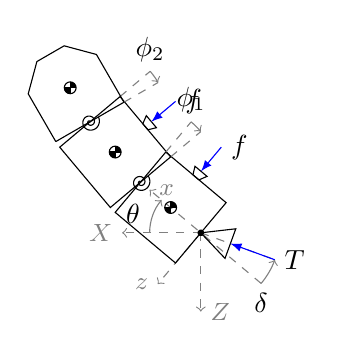
\begin{tikzpicture}[scale=1]
  
%Nodes

%Connectio
	\draw[axis,->]  (0,0) -- (0,-1)  node[right]{$Z$};
	\draw[axis,->]  (0,0) --  (-1,0) node[left]{$X$};
	\draw[draw=gray,->,] (-0.65,0) node[above left]{$\theta$} arc (180:140:0.65);
	
	\begin{scope}[yshift=0cm,rotate=50]
	\draw[axis,->]  (0,-1) -- (0,0.85)  node[right]{$x$};
	\draw[axis,->]  (0,0) --  (-0.85,0) node[left]{$z$};
	\draw[] (-0.5,0) rectangle (0.5,1);
	\node[cog] at (0,0.5) {};
	\draw[draw=gray,->,] (1,1) node[above]{$\phi_1$} arc (0:-10:1);
	
	\draw[]  (0.5,0.45) -- (0.6,0.4) -- (0.6,0.6) --(0.5,0.55)-- cycle;
	\draw[force,->] (1,0.5)  node[right]{$f$}  -- (0.6,0.5);
	
	\begin{scope}[yshift=1cm,rotate=-10]
	\draw[axis,-]  (0.5,1) -- (1,1);
	\draw[axis,-]  (0.5,0) -- (1,0);
	\draw[] (-0.5,0) rectangle (0.5,1);
	\node[cog] at (0,0.5) {};
	\draw [domain=0:12.56,variable=\t,smooth,samples=75] plot ({\t r}: {0.010*\t});
	\draw[draw=gray,->,] (1,1) node[above]{$\phi_2$} arc (0:-10:1);
	
	\draw[]  (0.5,0.45) -- (0.6,0.4) -- (0.6,0.6) --(0.5,0.55)-- cycle;
	\draw[force,->] (1,0.5)  node[right]{$f$}  -- (0.6,0.5);
	
	\begin{scope}[yshift=1cm,rotate=-10]
	\draw[axis,-]  (0.5,0) -- (1,0);
	\draw[] (-0.5,0) -- (-0.5,0.7) -- (-0.2,1) -- (0.2,1) -- (0.5,0.7) -- (0.5,0) --  (-0.5,0) ;
	\node[cog] at (0,0.5) {};
	\draw [domain=0:12.56,variable=\t,smooth,samples=75] plot ({\t r}: {0.010*\t});
	
	\end{scope}
	\end{scope}
	
	\draw[axis,-]  (0.5,1) -- (1,1);
	\begin{scope}[rotate = 20]
	\draw[]  (0,0) -- (-0.2,-0.4) -- (0.2,-0.4) -- cycle;
	\draw[axis,-]  (0,0) -- (0,-1);
	\draw[force,->] (0,-1)  node[right]{$T$}  -- (0,-0.4);
	\filldraw (0,0) circle (1pt);
	\end{scope}
	\draw[draw=gray,->,] (0,-1) node[below]{$\delta$} arc (-90:-70:1);

	\end{scope}


\end{tikzpicture}